\documentclass{article}
\usepackage{listings}
\usepackage{color}
\usepackage{amsmath}
\usepackage{amsfonts}
\usepackage{amssymb}
\usepackage{caption}
\usepackage{polski}
\usepackage{indentfirst}
\usepackage{graphicx}
\usepackage{pdfpages}
\usepackage{gauss}

\DeclareCaptionType{equ}[][List of equations]
\captionsetup[equ]{labelformat=empty}

%script adding bars in matrix
\usepackage{etoolbox}
\makeatletter
\patchcmd\g@matrix
 {\vbox\bgroup}
 {\vbox\bgroup\normalbaselines}% restore the standard baselineskip
 {}{}
\makeatother

\newcommand{\BAR}{%
  \hspace{-\arraycolsep}%
  \strut\vrule % the `\vrule` is as high and deep as a strut
  \hspace{-\arraycolsep}%
}
\definecolor{dkgreen}{rgb}{0,0.6,0}
\definecolor{gray}{rgb}{0.5,0.5,0.5}
\definecolor{mauve}{rgb}{0.58,0,0.82}

\lstset{frame=tb,
  language=Python,
  aboveskip=3mm,
  belowskip=3mm,
  showstringspaces=false,
  columns=flexible,
  basicstyle={\small\ttfamily},
  numbers=none,
  numberstyle=\tiny\color{gray},
  keywordstyle=\color{blue},
  commentstyle=\color{dkgreen},
  stringstyle=\color{mauve},
  breaklines=true,
  breakatwhitespace=true,
  tabsize=3,
  extendedchars=\true,
  inputencoding=utf8x
}

\lstset{literate={ą}{{\k{a}}}1 {ł}{{\l{}}}1 {ń}{{\'n}}1 {ę}{{\k{e}}}1 {ś}{{\'s}}1 {ż}{{\.z}}1 {ó}{{\'o}}1 {ź}{{\'z}}1 {Ą}{{\k{A}}}1 {Ł}{{\L{}}}1 {Ń}{{\'N}}1 {Ę}{{\k{E}}}1 {Ś}{{\'S}}1 {Ż}{{\.Z}}1 {Ó}{{\'O}}1 {Ź}{{\'Z}}1 }

\begin{document}
\title{Sprawozdanie - Metody numeryczne i optymailzacja}
\author{Jakub Andryszczak 259519,\\ Jakub Żak 244255,\\ Maciej Cierpisz 249163}
\date{}
\maketitle

\newpage
\tableofcontents
%Tutaj zaczyna się wstęp

\newpage
\section{Zadanie nr. 1}
Znajdź liczby x1 i x2, które maksymalizują sumę x1 + x2 przy ograniczeniach:
\begin{equation}
    \begin{cases}
      x_{1} \geq 0,x_{2}\geq 0 \\
     x_{1}+2x_{2} \leq 2 \\
     4x_{1} + 2x_{2}\leq 12\\
     -x_1 + x_2 \leq 1, 
    \end{cases}\,.
  \end{equation}
  Narysować zbiór dopuszczalnych rozwiązań na $\Re^2$ i znaleźć rozwiązanie w ujęciu
geometrycznym, formułując zadanie programowania liniowego.
\newline

Początkowo zapisano wszystkie nierówności w formie równań z dodatkową niewiadomą,
\begin{equation}
    \begin{cases}
      x_{1}+2x_{2}+x_3 = 2 \\
     4x_{1} + 2x_{2}+x_4 = 12\\
     -x_1 + x_2 + x_5 = 1, 
    \end{cases}
  \end{equation}
Następnie wyświetlono wszystkie proste na jednym wykresie.
\begin{figure}[h]
    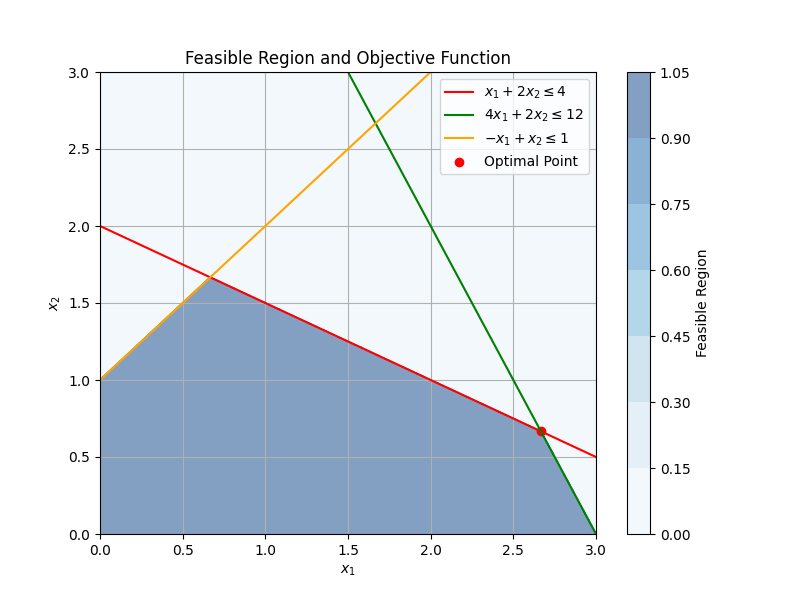
\includegraphics[scale=0.7]{Simplex1.png}
    \centering
    \captionsetup[Tabela]{name=New Table Name}
    \caption*{Wykres.2.1. Zależność n-tej iteracji metody do błędu residualnego}
  \end{figure}
\section{Zadanie nr. 2}

\section{Zadanie nr. 3}

\section{Zadanie nr. 4}
W pewnej rafinerii proces rafinacji wymaga wyprodukowania co najmniej dwóch
litrów benzyny na każdy litr oleju opałowego. Aby sprostać przewidywanemu zapotrzebowaniu
w okresie zimowym, trzeba będzie produkować co najmniej trzy miliony litrów oleju
opałowego dziennie. Z kolei, zapotrzebowanie na benzynę wynosi nie więcej niż 6,4 miliona
litrów dziennie. Jeśli benzynę sprzedaje się po 1,90 dolara za litr, a olej opałowy po 1,50 dolara
za litr, to ile należy wyprodukować każdego z tych produktów, aby zmaksymalizować
przychody?
\newline

Aby rozwiązać zadania, sformułowano funkcję celu, którą chcemy zmaksymalizować. Dla $x_1$ oznaczamy litry oleju opałowego, 
a $x_2$ litry benzyny, które należy wyprodukować. Przychody można obliczyć jako iloczyn ilości litrów każdego produktu i odpowiadających im cen:
\begin{equation}
   f(x_1,x_2)=1.5x_1 + 1.9x_2 
\end{equation}

Należy wyprodukować co najmniej trzy miliony litrów oleju opałowego, a proces rafinacji wymaga wyprodukowania co najmniej dwóch litrów
benzyny na każdy litr oleju opałowego, a ograniczenie zapotrzebowania na benzynę wynosi nie więcej niż 6,4 miliona litrów dziennie, więc
\begin{equation}
    \begin{cases}
        x_1 \geq 3000000\\
        x_2 \leq 6 400 000\\
        -2x_1 + x_2 \geq 0
    \end{cases}
\end{equation}
\section{Zadanie nr. 5}

\section{Zadanie nr. 6}

\end{document}